\documentclass[11pt,a4paper]{article}
\usepackage[a4paper, hmargin={2.5cm,2.5cm},vmargin={2.5cm,2.5cm}]{geometry}
\usepackage{graphicx}
\usepackage{cmap}
\usepackage[utf8]{inputenc}
\usepackage[english]{babel}
\usepackage{amsmath}
\usepackage{amsfonts}
\usepackage{listings}
\usepackage{color}
\usepackage{pdfpages}
\usepackage{fancyvrb}
\usepackage{fancyhdr}
\usepackage{lipsum}
% \usepackage{pgfplots}
\usepackage{wrapfig}
\usepackage{subfig}
\usepackage{enumitem}
\usepackage{tikz}
\usepackage{forest}


\usetikzlibrary{automata, positioning, arrows}
\usetikzlibrary{positioning}
\usetikzlibrary{shapes,shapes.geometric,arrows,fit,calc}

\def\dunderline#1{\underline{\underline{#1}}}
\def\indent{\space\space\space\space}

\begin{document}
\begin{titlepage}
  \title{Programmer som data trial exam}
  \author{Albert Ross Johannessen}
  \maketitle
  \newpage
  \thispagestyle{empty}
  \newpage
\end{titlepage}

\pagestyle{fancy}
\fancyhf{}
\rhead{Programmer som data}
\rfoot{Page \thepage}
\newpage
\section{}
Betragt den ikke-deterministiske endelige automat (''nondeterministic finite automaton'', NFA) nedenfor. Det anvendte alfabet er $\lbrace a,b\rbrace$. Der er i alt 5 tilstande, hvor tilstand 5 er den eneste accepttilstand.
\begin{figure}[!ht]\label{fig:examfignfa}
    \centering
    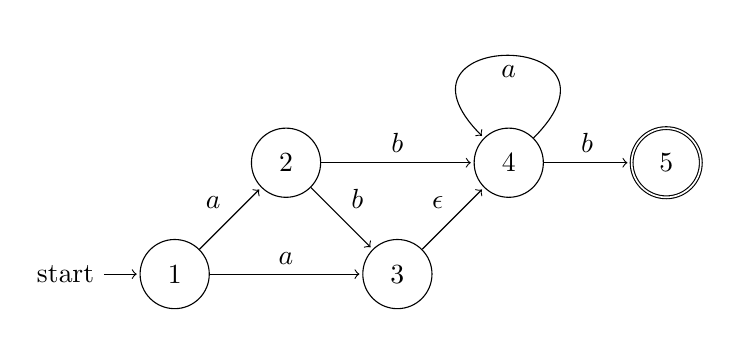
\begin{tikzpicture}[shorten >=1pt,node distance=2cm,on grid,auto] 
       \node[state, initial] (q_1)   {$1$}; 
        \node[state] (q_2) [above right =of q_1] {$2$};
        \node[state] (q_3) [below right =of q_2] {$3$};
        \node[state] (q_4) [above right =of q_3] {$4$};
        \node[state,accepting] (q_5) [ right =of q_4] {$5$};
              
        \path[->] 
        (q_1) edge  node {$a$} (q_2)
        (q_1) edge  node {$a$} (q_3)
        (q_2) edge  node {$b$} (q_3)
        (q_2) edge  node {$b$} (q_4)
        (q_3) edge  node {$\epsilon$} (q_4)
        (q_4) edge [loop] node {$a$} (q_4)
        (q_4) edge  node {$b$} (q_5)
        ;
    \end{tikzpicture}
    \caption{The labeled NFA}
\end{figure}
\subsection{Angiv alle årsager til at automaten er ikke-deterministisk}
\begin{itemize}
  \item Fra knude $1$ er der $2$ $a$ kanter.
  \item Fra knude $2$ er der $2$ $b$ kanter.
  \item Fra knude $3$ er der èn $\epsilon$ kant.
\end{itemize}
\subsection{Giv tre eksempler på strenge der genkendes af automaten}
\begin{itemize}
  \item abb
  \item abaaaab
  \item aaaaaab
\end{itemize}
\subsection{Giv en uformel beskrivelse af sproget (mængden af all strenge) der beskrives af automaten}
\begin{itemize}
  \item Der er to måder at starte på denne automat.
  \begin{enumerate}
    \item Ét $a$ og herefter ét $b$.
    \item Ét eller flere $a$.
  \end{enumerate}
  Herefter er slutningen ens man kan vælge et vilkårligt antal $a$ og herefter \textbf{skal} man slutte af på ét $b$. Kanten fra $2$ til $3$ er overflødig og det samme er knude $3$, hvis man sætter en kant mellem $1$ og $4$.
\end{itemize}
\subsection{Konstruer og tegn en deterministisk endelig automat}
Konstruer og tegn en deterministisk endelig automat (''deterministic finite automaton'', DFA) der svarer til automaten ovenfor. Husk at angive starttilstand og accepttilstand (e). Du skal enten bruge en systematisk konstruktion svarende til den i forelæsningen eller som i Introduction to Compiler Design (ICD), eller Basics of Compiler Design (BCD), eller forklare hvorfor den resulterende automat er korrekt.\\
Vi starter med at konstruerer vores subset.
\newpage
\begin{figure}[!ht]\label{fig:nfa2dfa}
  \centering
  \begin{tabular}{c|ccc}
          & $a$ & $b$ & NFA State\\\hline
    $S_1$ & $\left\{2, 3,4\right\}^{S_2}$ & $\left\{\right\}$ & $\left\{1\right\}$ \\
    $S_2$ & $\left\{4\right\}^{S_3}$ & $\left\{3,4,5\right\}^{S_4}$ & $\left\{2,3,4\right\}$\\
    $S_3$ & $\left\{\right\}^{S_3}$ & $\left\{5\right\}^{S_5}$ & $\left\{4\right\}$\\
    $S_4$ & $\left\{\right\}^{S_3}$ & $\left\{5\right\}^{S_5}$ & $\left\{3,4,5\right\}$\\
    $S_5$ & $\left\{\right\}$ & $\left\{\right\}$ & $\left\{5\right\}$
  \end{tabular}
\end{figure}
\noindent Dette giver følgende DFA, vi skal dog verificere at den er minimal.
\begin{figure}[!ht]\label{fig:examfigdfa}
    \centering
    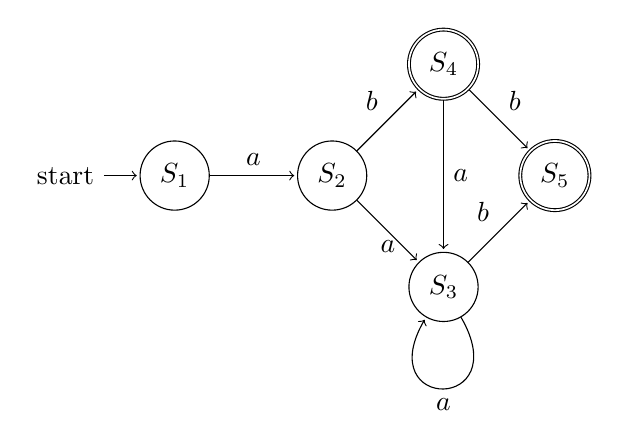
\begin{tikzpicture}[shorten >=1pt,node distance=2cm,on grid,auto] 
       \node[state, initial] (s_1)   {$S_1$}; 
        \node[state] (s_2) [right =of s_1] {$S_2$};
        \node[state] (s_3) [below right =of s_2] {$S_3$};
        \node[state, accepting] (s_4) [above right =of s_2] {$S_4$};
        \node[state, accepting] (s_5) [above right =of s_3] {$S_5$};
              
        \path[->] 
        (s_1) edge  node {$a$} (s_2)
        (s_3) edge [in=240, out=300,loop] node {$a$} (s_3)
        (s_2) edge node [below]{$a$} (s_3)
        (s_2) edge node {$b$} (s_4)
        (s_4) edge  node {$a$} (s_3)
        (s_4) edge  node {$b$} (s_5)
        (s_3) edge node {$b$} (s_5)
        ;
    \end{tikzpicture}
    \caption{The labeled DFA}
\end{figure}\\
Vi starter med at tjekke om grupperne er konsistente.
\begin{figure}[!ht]\label{fig:mindfa:gs}
  \centering
  \begin{tabular}{c|c}
    $G_1$ & $\left\{S_1, S_2, S_3\right\}$\\
    $G_2$ & $\left\{S_4, S_5\right\}$
  \end{tabular}
\end{figure}
\begin{figure}[!ht]\label{fig:mindfa:g1}
  \centering
  \begin{tabular}{c|cc}
    $G_1$ & $a$ & $b$\\\hline
    $S_1$ & $\left\{G_1\right\}$ & -\\
    $S_2$ & $\left\{G_1\right\}$ & $\left\{G_2\right\}$\\
    $S_3$ & $\left\{G_1\right\}$ & $\left\{G_2\right\}$
  \end{tabular}
\end{figure}\\
$G_1$ er ikke konsistent så vi opretter 2 nye grupper.
\begin{figure}[!ht]\label{fig:mindfa:newgs}
  \centering
  \begin{tabular}{c|c}
    $G_2$ & $\left\{S_4, S_5\right\}$\\
    $G_3$ & $\left\{S_1\right\}$\\
    $G_4$ & $\left\{S_2, S_3\right\}$
  \end{tabular}
\end{figure}\\
\begin{figure}[!ht]\label{fig:mindfa:g2}
  \centering
  \begin{tabular}{c|cc}
    $G_2$ & $a$ & $b$\\\hline
    $S_4$ & $\left\{G_4\right\}$ & $\left\{G_2\right\}$ \\
    $S_5$ & - & -
  \end{tabular}
\end{figure}\\
\begin{figure}[!ht]\label{fig:mindfa:newgs}
  \centering
  \begin{tabular}{c|c}
    $G_3$ & $\left\{S_1\right\}$\\
    $G_4$ & $\left\{S_2, S_3\right\}$\\
    $G_5$ & $\left\{S_4\right\}$\\
    $G_6$ & $\left\{S_5\right\}$
  \end{tabular}
\end{figure}\\
\begin{figure}[!ht]\label{fig:mindfa:g3}
  \centering
  \begin{tabular}{c|cc}
    $G_3$ & $a$ & $b$\\\hline
    $S_1$ & $\left\{G_4\right\}$ & -
  \end{tabular}
\end{figure}\\
\begin{figure}[!ht]\label{fig:mindfa:g4}
  \centering
  \begin{tabular}{c|cc}
    $G_4$ & $a$ & $b$\\\hline
    $S_2$ & $\left\{G_4\right\}$ & $\left\{G_5\right\}$\\
    $S_3$ & $\left\{G_4\right\}$ & $\left\{G_6\right\}$
  \end{tabular}
\end{figure}\\
\begin{figure}[!ht]\label{fig:mindfa:newgs}
  \centering
  \begin{tabular}{c|c}
    $G_3$ & $\left\{S_1\right\}$\\
    $G_5$ & $\left\{S_4\right\}$\\
    $G_6$ & $\left\{S_5\right\}$\\
    $G_7$ & $\left\{S_2\right\}$\\
    $G_8$ & $\left\{S_3\right\}$\\
  \end{tabular}
\end{figure}\\
There are only singletons left, this means that we have a minimal DFA.
\subsection{Angiv et regulært udtryk}
Angiv et regulær udtryk der beskriver mængden af strenge over alfabete $\left\{a, b\right\}$, som beskrives af automaten ovenfor. Check og forklar at det regulære udtryk også beskriver mængden af strenge for din DFA.
\begin{align}
  ab?a*b
\end{align}
\end{document}
